% Copyright (C) 2014-2017 by Thomas Auzinger <thomas@auzinger.name>

\documentclass[draft,final]{vutinfth} % Remove option 'final' to obtain debug information.

% Load packages to allow in- and output of non-ASCII characters.
\usepackage{lmodern}        % Use an extension of the original Computer Modern font to minimize the use of bitmapped letters.
\usepackage[T1]{fontenc}    % Determines font encoding of the output. Font packages have to be included before this line.
\usepackage[utf8]{inputenc} % Determines encoding of the input. All input files have to use UTF8 encoding.

% Extended LaTeX functionality is enables by including packages with \usepackage{...}.
\usepackage{amsmath}    % Extended typesetting of mathematical expression.
\usepackage{amssymb}    % Provides a multitude of mathematical symbols.
\usepackage{mathtools}  % Further extensions of mathematical typesetting.
\usepackage{microtype}  % Small-scale typographic enhancements.
\usepackage[inline]{enumitem} % User control over the layout of lists (itemize, enumerate, description).
\usepackage{multirow}   % Allows table elements to span several rows.
\usepackage{booktabs}   % Improves the typesettings of tables.
\usepackage{subcaption} % Allows the use of subfigures and enables their referencing.
\usepackage[ruled,linesnumbered,algochapter]{algorithm2e} % Enables the writing of pseudo code.
\usepackage[usenames,dvipsnames,table]{xcolor} % Allows the definition and use of colors. This package has to be included before tikz.
\usepackage{nag}       % Issues warnings when best practices in writing LaTeX documents are violated.
\usepackage{todonotes} % Provides tooltip-like todo notes.
\usepackage{hyperref}  % Enables cross linking in the electronic document version. This package has to be included second to last.
\usepackage[acronym,toc]{glossaries} % Enables the generation of glossaries and lists fo acronyms. This package has to be included last.

% Define convenience functions to use the author name and the thesis title in the PDF document properties.
\newcommand{\authorname}{Bernhard Gößwein} % The author name without titles.
\newcommand{\thesistitle}{Designing a Framework gaining Repeatability for the OpenEO platform} % The title of the thesis. The English version should be used, if it exists.

% Set PDF document properties
\hypersetup{
    pdfpagelayout   = TwoPageRight,           % How the document is shown in PDF viewers (optional).
    linkbordercolor = {Melon},                % The color of the borders of boxes around crosslinks (optional).
    pdfauthor       = {\authorname},          % The author's name in the document properties (optional).
    pdftitle        = {\thesistitle},         % The document's title in the document properties (optional).
    pdfsubject      = {Subject},              % The document's subject in the document properties (optional).
    pdfkeywords     = {a, list, of, keywords} % The document's keywords in the document properties (optional).
}

\setpnumwidth{2.5em}        % Avoid overfull hboxes in the table of contents (see memoir manual).
\setsecnumdepth{subsection} % Enumerate subsections.

\nonzeroparskip             % Create space between paragraphs (optional).
\setlength{\parindent}{0pt} % Remove paragraph identation (optional).

\makeindex      % Use an optional index.
\makeglossaries % Use an optional glossary.
%\glstocfalse   % Remove the glossaries from the table of contents.

% Set persons with 4 arguments:
%  {title before name}{name}{title after name}{gender}
%  where both titles are optional (i.e. can be given as empty brackets {}).
\setauthor{}{\authorname}{}{male}
\setadvisor{Ao.Univ.Prof. Dipl.-Ing. Dr.techn.}{Andreas Rauber}{}{male}

% For bachelor and master theses:
%\setfirstassistant{Ao.Univ.Prof. Dipl.-Ing. Dr.techn.}{Andreas Rauber}{}{male}
\setfirstassistant{Dr.}{Tomasz Miksa}{}{male}
%\setthirdassistant{Pretitle}{Forename Surname}{Posttitle}{male}

% For dissertations:
%\setfirstreviewer{Pretitle}{Forename Surname}{Posttitle}{male}
%\setsecondreviewer{Pretitle}{Forename Surname}{Posttitle}{male}

% For dissertations at the PhD School and optionally for dissertations:
%\setsecondadvisor{Pretitle}{Forename Surname}{Posttitle}{male} % Comment to remove.

% Required data.
\setaddress{Vorderer Ödhof 1, 3062 Kirchstetten}
\setregnumber{01026884}
\setdate{01}{01}{2001} % Set date with 3 arguments: {day}{month}{year}.
\settitle{\thesistitle}{Deutscher Titel} % Sets English and German version of the title (both can be English or German). If your title contains commas, enclose it with additional curvy brackets (i.e., {{your title}}) or define it as a macro as done with \thesistitle.
\setsubtitle{}{} % Sets English and German version of the subtitle (both can be English or German).

% Select the thesis type: bachelor / master / doctor / phd-school.
% Bachelor:
%\setthesis{bachelor}
%
% Master:
\setthesis{master}
\setmasterdegree{dipl.} % dipl. / rer.nat. / rer.soc.oec. / master
%
% Doctor:
%\setthesis{doctor}
%\setdoctordegree{rer.soc.oec.}% rer.nat. / techn. / rer.soc.oec.
%
% Doctor at the PhD School
%\setthesis{phd-school} % Deactivate non-English title pages (see below)

% For bachelor and master:
\setcurriculum{Software Engineering and Internet Computing}{Software Engineering and Internet Computing} % Sets the English and German name of the curriculum.

% For dissertations at the PhD School:
%\setfirstreviewerdata{Affiliation, Country}
%\setsecondreviewerdata{Affiliation, Country}


\begin{document}

\frontmatter % Switches to roman numbering.
% The structure of the thesis has to conform to
%  http://www.informatik.tuwien.ac.at/dekanat

\addtitlepage{naustrian} % German title page (not for dissertations at the PhD School).
\addtitlepage{english} % English title page.
\addstatementpage

\begin{danksagung*}
\todo{Ihr Text hier.}
\end{danksagung*}

\begin{acknowledgements*}
\todo{Enter your text here.}
\end{acknowledgements*}

\begin{kurzfassung}
\todo{Ihr Text hier.}
\end{kurzfassung}

\begin{abstract}
\todo{Enter your text here.}
\end{abstract}

% Select the language of the thesis, e.g., english or naustrian.
\selectlanguage{english}

% Add a table of contents (toc).
\tableofcontents % Starred version, i.e., \tableofcontents*, removes the self-entry.

% Switch to arabic numbering and start the enumeration of chapters in the table of content.
\mainmatter

\chapter{Introduction}
\section{Problem Description}
Over the last decades remote sensing agencies have increased the variations of data processing and therefore the amount of resulting data. To preserve the data for further usage in the future it is necessary to have citable data and processes on the data to ensure repeatability in a long-term.\cite{6352411} 
Already most of the the data used in earth observation sciences are retrieved or provided via Service Oriented Architecture (SOA) interfaces. Provider like Google Earth Engine and EODC provide an Web API for retrieving and processing data. Due to a different range of functionality and a difference between the endpoints of the providers it is hard to create a workflow for more than one provider.  
The OpenEO project has the goal to be an abstraction layer above different EO data providers. The underlying structure consists of three parts:
\begin{itemize}
	\item Client Module : Is written in the program language of the user and transfers the users commands to the backends.
	\item Core Module: A standard on how the communication should take place between client and backend.
	\item Backend Module: The provider of the data and the services, which gets the instructions from the clients and returns the results.
\end{itemize}   
Further information on the software architecture of the project is defined in the project proposal (\cite{openeo}).Until now there is no consideration of repeatability verification of workflows for users in the OpenEO architecture.Generalised layers have the opportunity to be implemented in a way that makes processes and data scientifically verifiable and reproducible, because it handles data and processes on the data in a standardised way on different providers. Even though the range of functionality and the API endpoints are well defined in the OpenEO coreAPI the contributing content providers (OpenEO backends) will have different underlying software types and versions. The underlying technology of an OpenEO backend will also change over time and can lead to different results on the same workflow executions. Consider the following: A scientist runs an experiment using OpenEO as his research tool and gets results. The same scientist runs the same experiment with the same input some months later and gets slightly different results. The question occurs, why are the results different? Has the used data changed, has the user accidentally submitted different code or has some underlying software inside the backend provider changed. Adding a possibility for the users of OpenEO to gain this information is an important feature for the scientific community. The aim of this thesis is to provide a possibility for users of OpenEO to verify and validate a job re-execution on different underlying technologies of an OpenEO backend provider.\cite{openeo}
\todo{Read through and improve above text.}

\section{Aim of this Work}

The expected outcome of this thesis is to discover and develop a possible framework for providing repeatability in the OpenEO project. This enables users to re-execute workflows and validate the results, so that differences on the process or data are accessible for the users. To achieve this goal a model for repeatability within the project has to be discovered and implemented to evaluate the ability of the model. The model shall then conclude recommendations for the OpenEO project on how to improve re-execution validation for the user and how it can be achieved. Therefore the following research questions can be formulated:

\begin{itemize}
	\item \textbf{How can an OpenEO job re-executed be applied like the initial execution?}
	\begin{itemize}
		\item How can the used data be identified after the initial execution?
		\item How can the used software of the initial execution be reproduced?
		\item What data has to be captured when?
		\item How can the result of a re-execution in future software versions be verified?
	\end{itemize}
	\item \textbf{How can the equality of the OpenEO job re-execution results be validated?}
	\begin{itemize}
		\item What are the validation requirements?
		\item How can the data be compared?
		\item How can the re-execution be validated after changes of the OpenEO backend environment?
		\item How can differences in the environment between the executions be discovered?
	\end{itemize}
\end{itemize}
\todo{Read through above text and improve.}
\todo{Add description of use cases (see summary).}
\chapter{Related Work}
Currently, there exists no concrete solution to add the ability of repeatability to the OpenEO project. However there are concepts of adding repeatability in computer science.

\section{Reproducibility}
\subsection{eScience}
The eScience has the potential to enable a boost in scientific discovery by providing approaches to make digital data and workflows citable. In \cite{Rauber2015RepeatabilityAR} is a common way of reaching this goal formulated. It describes an approach to look at whole research processes, other than only data citation by introducing Process Management Plans. The capturing, verification and validation of the needed data for a computational process is also demonstrated within the paper.\cite{Rauber2015RepeatabilityAR}

\subsection{Data Citation}
Since the earth observation community use a high amount of satellite data and also within the OpenEO project a lot of big data sets are being used, there needs to be a solution to cite the used data in a workflow. The Research Data Alliance (RDA) working group on data citation provides a 14 step recommendation of data citation. It contains solutions not only for static, but also for dynamic data, so data that changes over time. Using the guideline for data citations from the RDA makes the data scientifically citable. \cite{rauber2016identification} 
In earth science there is also a strategy of ESA and NASA to achieve a content standard for data preservation.\cite{6352411}

\subsection{Provenance Data}
The re-execution of an OpenEO workflow not only needs data citation, but also the information of how the workflow was executed. Therefore provenance data has to be captured.\cite{Roure11towardsthe}There are already several provenance models defined in the scientific community. One of the existing models is the PROV model, which was published in 2013 by the World Wide Web Consortium Provenance Working Group and consists of recommendations and guidelines for provenance data.\cite{MOREAU2015235} 
Another model is the VFramework, designed for the purpose of redeployment including the verification of a re-execution of the same workflow. \cite{DBLP:conf/ipres/MiksaPMSVBR13}

\section{Related Work in the EO Sciences}

\section{Related Tools}
\todo{Read through above text and improve.}
\subsection{ReproZip}
\todo{Add section about ReproZip.}
\subsection{Smartcontainer}
\todo{Add section about Smartcontainer.}
\subsection{Reproducibility in computational geoscience}

\section{OpenEO Details}
The OpenEO project contains of three modules, the client modules written in the programming language of the users, the back end drivers that makes it possible for every backend to understand the calls from the clients and the core API that specifies how the communication should take place. So the core API is a standard that the back end providers accepted to implement on their systems. The back end drivers are the translation of the client calls to the back end specific API. This architecture decouples the clients from the back ends so that every client can connect to every back end that applies to the OpenEO core API standard see figure %#TODO.   

\begin{figure}[h]
	\centering
	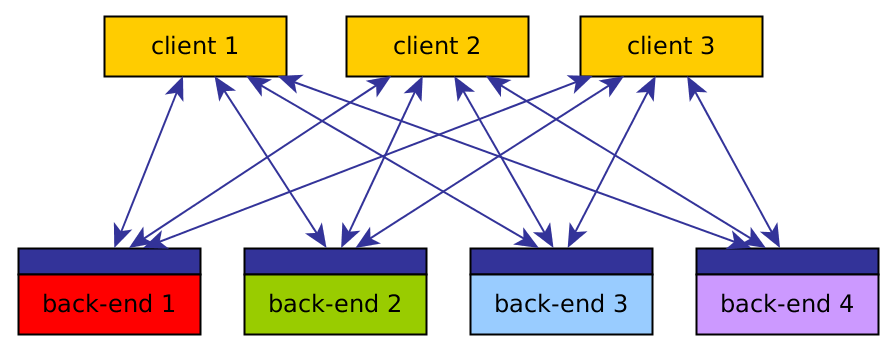
\includegraphics[width=\textwidth]{api2}
	\caption{Overview of the OpenEO architecture. (from openeo.org)}
	\label{fig:intro} % \label has to be placed AFTER \caption (or \subcaption) to produce correct cross-references.
\end{figure}


The communication is specified as an OpenAPI(TODO: Quelle) description and consists of all RESTful services that can be called at the back ends. Most of the calls are only to receive information about the processes and the data of the specific back end, but there are also endpoints to apply job executions specified by the user. In this thesis the focus lies on the job execution, because this is the core feature of the OpenEO project and needs to be reproducible. In the next chapter the job execution process is described in more detail. 

\subsection{Job Execution}
The job execution workflow in OpenEO starts at a client application that let the user define what has to be processed in the specific programming language.
The main part of the job execution is based on the description of what the back end needs to do with what data. Therefore OpenEO introduces the process graph, which consists of a tree structure describing the processes with their data and the input data identifier, which is back end specific. The process graph is in a JSON format and gets generated by the clients in the background without the users seeing it directly. In figure %#TODO there is an example of a process graph. 

\begin{figure}[h]
	\centering
	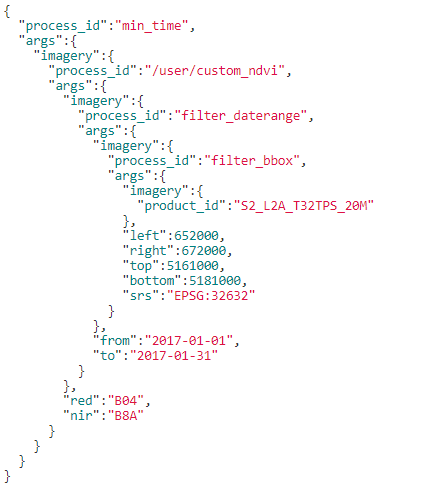
\includegraphics[width=\textwidth]{process_graph}
	\caption{Process graph example (from Github Spec)}
	\label{fig:intro} % \label has to be placed AFTER \caption (or \subcaption) to produce correct cross-references.
\end{figure}

The back ends interpret the process graph from inside out. Inside figure TODO the element in the middle defines the input data identifier in the \"imagery\" block, with the \"product\_id\". In this case the \"s2a\_prd\_msil1c\" is the chosen input data identifier. Now the back end goes one step up in the hierarchy of the process graph and calls the process \"filter\_bbox\" with the parameters \"left\", \"right\" and so on using the input data. The output data of the previous process is also the input data of the next process. It is possible that the input of a process is a whole new process graph. In figure %#TODO the same process graph is visualized from the back end point of view, so how it gets interpreted. 

\todo{Add Diagramm of Process Graph}

There are two different kinds of process executions depending on the back ends capabilities, synchronous and asynchronous calls. Synchronous calls are directly executed after they got received from the back end and the user that sends the process graph has to wait until the job is finished. For example on the python client the program waits after sending the process graph to the back end until the back end returns the result and the results are directly returned to the user. On the asynchronous call the user sends the process graph, but it does not get executed until the user starts the execution on the back end through an additional endpoint. When the processing is finished the user can download the result at another endpoint of the back end. For the asynchronous calls there is also the possibility to subscribe to a notification system on the backend, so that the user gets notified when the job execution finishes.     
The processes are defined at the OpenEO core API and therefore independent from the back end they get called, other than the data identifier, which is different for every back end.  
\\
The previous example shows a process graph that only uses predefined processes and data. Within the OpenEO project there is the possibility to define individual processes and execute them on the back end. In the project they are called “user defined functions” and are at the writing of this thesis not well defined, but are basically code written by the OpenEO user that gets sent to the back end and executed at a secure environment. The user can define processes and can run them with the data provided at the back end, using the infrastructure of the back end. Every back end has to individually define what the restrictions on user defined functions are. 
There is also the possibility to upload files to the back end that can be used within the process graph. The user can upload the file through an explicit endpoint of the back end. After the upload finished, the file can be referenced inside the process graph.   % [#TODO: Quelle Github Docu Release Version 0.0.2]

\subsection{Back end Overview}
Even though the back ends implement the OpenEO core API standard, they are still very diverse behind the abstraction layer. Some back ends has already an API, where the OpenEO calls have to be adapted to. There are 7 partners within the OpenEO project that are implementing a back end driver. The back ends have to manage the translation of the process graph to the actual code that executes the defined process chain. Also the billing of the users is completely different on every back end. 
%#TODO: Explain different back ends → neccessary in detail ?
%#TODO: Explain execution of jobs in the back end. (Translation of Process Graph to Code)


\todo{Add section about EO reproducibility.}
\chapter{Design}
In this chapter the design of the provenance capturing gets described. First the architecture of the OpenEO project gets described further. Especially the job execution path throughout the parts of OpenEO gets described, because it is the key element for the context capturing. Therefore the back end, where the jobs get executed get described in more detail. After that the context model gets presented. %#TODO: Rewrite

In this section the concept of the provenance capturing is described. The aim of the capturing is to be easy to implement on the OpenEO back ends, but also powerful enough to make the reproduction of the workflows possible. The whole capturing process can be structured in three thematic parts.
\begin{enumerate}
	\item \textbf{Back end provenance} \\
	This part describes the provenance of the back end, that is not depending on a job execution. There has to be an automated process running on the process machine to capture every change that influences the execution of OpenEO jobs. A description of more detail can be viewed on chapter %#TODO.  
	\item\textbf{Job dependent provenance} \\
	This part contains the provenance of a job execution. It consists of the workflow context and the data related to one specific job. This in combination of the back end provenance is the full provenance data to make an OpenEO job theoretically re-executable.
	\item \textbf{User information} \\
	This part consists of all possibilities that provides users with information they want to know about the provenance of the back end and the provenance of the job execution. The aim is to provide users with information that makes them easier to choose between back ends. On the other hand the user shall be able to retrieve the provenance data of the job in a way that the back end has no security risks. This part is not directly part of the context model, but of the implementation on the user interface.
\end{enumerate}
\section{Back end provenance}
The scope of this part of the context model is to get the static environment of where the job execution at the back end takes place. It contains the provenance data that is independent from a job execution, so does not change regardless of how much jobs were processed. It can only change from inside of the back ends by their maintainers. In the OpenEO project there are a great variety of different back end providers with very different setups, so the challenge of this part is to make it as simple and generic as possible. The data captured in this part of the context model is not meant to be shown to the user directly, because of security issues. The following data gets suggested to be the minimal set of static provenance data that has to be captured.
\begin{enumerate}
	\item \textbf{Github Repository} \\
	Since the project is an open source project and every back end has a github repository were at least the basic setup is stored. The aim of this strategy is to get other back ends with similar settings to reuse the already working setups of the running back ends.  Therefore, at least during the project runtime, every back end provider has a github repository were the code is publically available. This information is added to the back end provenance by saving the git repository url, the used branch, the used commit and local changes to the repository.
	\item\textbf{Used Folders} \\
	The back end will most probably not only use the github repository for the processing, so that other folders are involved that stores config files or additional code. This information is also crucial for the job execution and therefore needs to be stored. Changes of this directory have to be detected and stored in the context model. Temporary written folders have to be excluded to the capturing to prevent detecting changes that are not important. 
	\item \textbf{OS and packages} \\
	The operating system can also have an impact on the processing and so it has to be stored to the context model too. Not only the information about the operating system, but also the installed packages have to be stored in the context model. In a linux based system it is sufficient to store the location where the packages get installed (e.g. /etc). If the whole processing is done in a virtual container the operating system of that container shall be stored. If the whole processing is done in a docker container, the docker description file has to be saved in addition. But only if the docker container description does not change on different input process graphs, otherwise it has to be added to the “job dependent provenance”. 
	\item \textbf{Core API Version} \\
	The back ends core api version is the version of the OpenEO core API version it is using. In the productive usage of the OpenEO project it can happen, that the versions of the clients and the back ends differ, so that the behaviour might not compatible. So the back end server configuration is depending on the core API version of OpenEO, hence it shall be added to the context model. 
	\item \textbf{Back End Version} \\
	The captured data described in the previous sections will result in a back end version. The back end version shall be an identifier (e.g. a number) that gets updated on every change of the backend considering the provenance data described above. 
	
	To  provide long term stability of the capturing, there shall be a tool to automatically capture the provenance data to the context model. Every change on any of the previously described context data has to be detected automatically and have to result in a new back end version. This can be done by a standalone capturing tool that does not need to have detailed insights into the back end. 
	
\end{enumerate}
\section{Job dependent provenance}
In this section the job dependent provenance of the context model gets described. The data captured is tied to an specific job execution, so for every job execution a new context model gets created. The structure of the capturing is using the defined process graph structure of OpenEO. The process graph is already a description of the processes that run at the back end. So sending the same process graph to the same back end again shall result in the same outcome. To assure that the process graph results in the same way of processing the processing itself gets captured. After receiving the job the back end will transform the process graph into code that actually does the processing. Figure %#TODO shows the structure of the workflow capturing. 

%#TODO Overview Figure → maybe from the presentation of Wageningen
\begin{figure}[h]
	\centering
	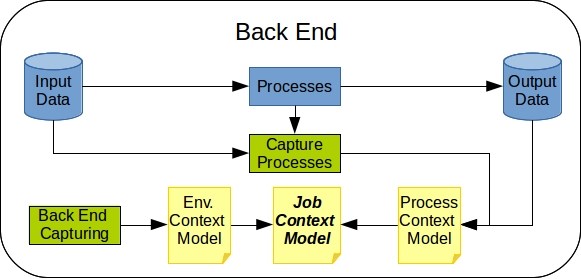
\includegraphics[width=\textwidth]{design_overview_common}
	\caption{Design Overview of capturing the job context model.}
	\label{fig:intro} % \label has to be placed AFTER \caption (or \subcaption) to produce correct cross-references.
\end{figure}

The single parts of the capturing are described more in detail in the following sections. 

\subsection{Input Data}
The input data of the processing is crucial for the outcome of the process graph. Even though the process graph already uses an identifier for the input data that has to be unique for the specific back end, changes to this data might not result in a new identifier. So jobs called later in time might use another version of the input data than the previous jobs. To prevent this the input data has to be persisted according to the 14 steps of data provenance defined by the RDA[1] described in the related work section. Every back end is responsible for the data versioning, for this context model it is assumed that the back ends preserve the data properly. Nevertheless the current core API version (v0.0.2) is not capable of letting the user choose, which version of data the user want to use. Hence there has to be an addition to the process graph so that product identifier shall have an additional timestamp. The meaning of the timestamp is to tell the back end that the user wants to use the data at the time of the timestamp. This gives the back ends the possibility to design their own data versioning. They just have to remember, which version of the data was available on what date and time. 
Not only the product used for the process graph is input data but also files uploaded by the user are included at the input data. As long as the file name is accessed at the specific process graph the file gets added to the provenance of the job execution. 

To guarantee that the data has not changed even though the version has not changed it is considered that a hash of the input data is added to the provenance data. The earth observation data stored at the OpenEO back ends can be very big and therefore it is recommended that the back end provider already hash the input data after every change on it so that the performance of the job execution is not threatened. This also applies to the uploaded files of the user, where the hash can be done already after the uploading. In OpenEO files that get uploaded with the same filename are automatically overwritten so that it is especially important to take the hash of this files for the context model. Otherwise it is not possible to replicate differences on a job execution. 

\subsection{Process Data}
In this section the capturing of the process itself gets described. As mentioned above the process is described at the process graph, but to be certain that the same process id results in the same code, the code has to be captured. So the code running the processing has to be captured and has to result in a signature that can be compared to other executions. An example of doing so is to hash the entire resulting code. 
The way of executing a specific process graph is not only related to the code running it, but also by the dependencies of the code. So the environment of the code and information about the code environment has to be added to the context model. If there are any docker container, where the job is running that is not independent on the process graph has to be captured. The programming language, its version and its used packages has also to be captured and added to the job context model. To every process executed also the start time and end time has to be captured as a time stamp.


\subsection{Output Data}
The output data of the processing has to be captured as well. In the OpenEO project the results can be rather big, that is why a simple generated identifier of the output result is enough in this context model. An example of this identifier would be a hash over the resulting data. The aim of the output data capturing is not to add the possibility to find differences between results, but to be able to see that the results are different. So for this context model a simple solution is sufficient. 

\subsection{Benchmarking}

So far only the capturing of a single process, including input and output data, are described, but not how the whole process graph shall be captured. The basic idea of the job dependent provenance capturing is to capture the input data of the process graph, the whole process graph and the output of the process graph, described like in the sections above. This is a common basis the back end providers can agree on and is not affecting the back end providers implementations much. It is also capable of giving the OpenEO user a simple overview of how the results are generated and what are differences between different job executions. 
To make the comparison of different execution behaviors more informative, the granularity of the capturing can be improved. 
\begin{figure}[h]
	\centering
	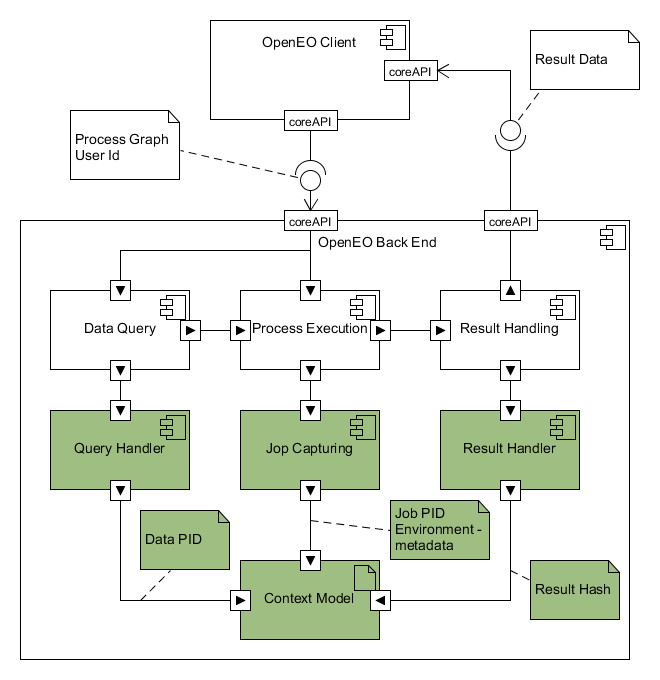
\includegraphics[width=\textwidth]{design_overview}
	\caption{Design Overview of capturing the job context model.}
	\label{fig:intro} % \label has to be placed AFTER \caption (or \subcaption) to produce correct cross-references.
\end{figure}
So that is how the benchmarking context model gets introduced. The idea is that not only the input data the whole process and the output data gets captured, but also every data in between of every process in the process graph. So for every process in the process graph the input, output data gets captured and the code executing the process. This makes it easier for users to see were the execution actually changed. But it also comes with higher implementation costs at the back end side. It also will affect the performance of the execution more than the common context model. The possibility of the implementation of such a granularity is also highly dependent on the back end implementation. Not every back end might be able to implement this into the back end due to execution optimization where the execution and results of the single  processes in the process graph are not distinctable. Nevertheless in theory the granularity does not have to stop there, the data and code could be captured for every line in the code. This flexibility of capturing makes it also a context model that  can be adapted to different use cases in the future. 
\section{User Information}

In this section the information for the users get described. The capturing described in the previous sections consists of a lot of  information about the back ends that shall not be passed to the users in detail. On the other hand the users need to be able to see the differences of job executions and get environment information about the backends. Therefore there has to be a filter on which data can be shown to the user and what not. Every captured information is also not necessary interesting for the users. Data that is not secure to the user has to be defined by the different back ends themselves. The OpenEO project has a very diverse kinds of back ends and every one has a unique company security guideline. The important thing is that all of the information has to be captured and taken into account for the comparisons and they have to be open to the user, but anonymously if needed.
The information has to be able to be provided to the user. Therefore there have to be some new additions to to the core api specification to do so. So there has to be a new endpoint for  the users to get information about the back end job independently. Therefore for this thesis the endpoint "GET /version" gets introduced, where the context model of the back end gets provided. 
There needs to be an endpoint to retrieve the job dependent provenance data, which can be added to the already existing "GET /jobs/<job\_id>" endpoint, which is used to get the current status information of the job. The endpoint also includes the back end provenance of the back end during the execution of the job. 
There shall be an additional endpoint for comparing two different jobs by their captured context model. For this purpose the endpoint "POST /jobs/<job\_id>/diff" gets introduced, were the job ids that the user wants to compare with are submitted by the POST body. 

\section{Overview of OpenEO Suggestions}
In this section the changes described in this chapter get summarized and assigned to the parts of OpenEO responsible for the tasks.

\subsection{OpenEO back end}
The openeo back ends need to implement the job dependent capturing as described in the section TODO and implemented in section TODO. The job dependent capturing is recommended to be implemented in the same programming language as the back end provider uses. The advantage of this is that the usage of the programming language is maintained anyway by the back ends to preserve the functionality of the processes and if the back end switches to a different location the setup of the capturing tool needs no further effort. 
The back end also need to run the job independent capturing described in section TODO. This has to be run in a cron job or other automation tools so that the changes get notices by the tool. In section TODO there is also an implemented tool doing so. 
In addition the backends need to implement the endpoints changes and additions of the OpenEO core API described in the next section.   
\subsection{OpenEO core API}
The core API needs to add the endpoint for the version retrieval (e.g. a /version) end point. It is also possible to extend an existing endpoint for this purpose. 
There needs also an additional endpoint for comparing two different jobs. 
The process graph shall be extended by a timestamp to the product element so that it is possible to access deprecated data on the back ends.
\subsection{OpenEO Client}
The OpenEO clients need to implement the changes described above in the core API additions. In the OpenEO client the additional retrieved data needs to be visualized for a better user understanding.


\todo{Read through above text and improve.}
\todo{Add section about noworkflow}
\chapter{Implementation}
\section{The EODC Backend}
\section{Job Independent Context}
\section{Job Dependent Context}
\section{User Interface}
\section{Overview of Changes}

\todo{Enter your text here.}

\chapter{Evaluation}
\section{Use Cases}
\section{Using Python Client}
\section{Performance Comparison}

\chapter{Conclusion and future Work}

\todo{Enter your text here.}

% Remove following line for the final thesis.
%%% intro.tex
%% Copyright (C) 2014-2017 by Thomas Auzinger <thomas@auzinger.name>
%
% This work may be distributed and/or modified under the
% conditions of the LaTeX Project Public License, either version 1.3
% of this license or (at your option) any later version.
% The latest version of this license is in
%   http://www.latex-project.org/lppl.txt
% and version 1.3 or later is part of all distributions of LaTeX
% version 2005/12/01 or later.
%
% This work has the LPPL maintenance status `maintained'.
%
% The Current Maintainer of this work is Thomas Auzinger.
%
% This work consists of the files vutinfth.dtx and vutinfth.ins
% and the derived file vutinfth.cls.
% This work also consists of the file intro.tex.


\newacronym{ctan}{CTAN}{Comprehensive TeX Archive Network}
\newacronym{faq}{FAQ}{Frequently Asked Questions}
\newacronym{pdf}{PDF}{Portable Document Format}
\newacronym{svn}{SVN}{Subversion}
\newacronym{wysiwyg}{WYSIWYG}{What You See Is What You Get}

\newglossaryentry{texteditor}
{
  name={editor},
  description={A text editor is a type of program used for editing plain text files.}
}

\chapter{Introduction to \LaTeX}

Since \LaTeX\ is widely used in academia and industry, there exists a plethora of freely accessible introductions to the language.
Reading through the guide at \url{https://en.wikibooks.org/wiki/LaTeX} serves as a comprehensive overview for most of the functionality and is highly recommended before starting with a thesis in \LaTeX.

\section{Installation}

A full \LaTeX\ distribution\index{distribution} consists of not only of the binaries that convert the source files to the typeset documents, but also of a wide range of packages and their documentation.
Depending on the operating system, different implementations are available as shown in Table~\ref{tab:distrib}.
\textbf{Due to the large amount of packages that are in everyday use and due to their high interdependence, it is paramount to keep the installed distribution\index{distribution} up to date.}
Otherwise, obscure errors and tedious debugging ensue.

\begin{table}
  \centering
  \begin{tabular}{cccc}
    \toprule
    Distribution & Unix         & Windows      & MacOS        \\
    \midrule
    TeX Live     & \textbf{yes} & yes          & (yes)        \\
    MacTeX       & no           & no           & \textbf{yes} \\
    MikTeX       & no           & \textbf{yes} & no           \\
    \bottomrule
  \end{tabular}
  \caption{\TeX/\LaTeX\ distributions for different operating systems. Recomended choice in \textbf{bold}.}
  \label{tab:distrib} % \label has to be placed AFTER \caption to produce correct cross-references.
\end{table}

\section{Editors}

A multitude of \TeX\ \glspl{texteditor} are available differing in their editing models, their supported operating systems and their feature sets.
A comprehensive overview of \glspl{texteditor} can be found at the Wikipedia page  \url{https://en.wikipedia.org/wiki/Comparison_of_TeX_editors}.
TeXstudio (\url{http://texstudio.sourceforge.net/}) is recommended.
Most editors support the scrolling the typeset preview document to a location in the source document by \verb|Ctrl| clicking the location in the source document.

\section{Compilation}

Modern editors usually provide the compilation programs to generate \gls{pdf} documents and for most \LaTeX\ source files, this is sufficient.
More advanced \LaTeX\ functionality, such as glossaries and bibliographies, needs additional compilation steps, however.
It is also possible that errors in the compilation process invalidate intermediate files and force subsequent compilation runs to fail.
It is advisable to delete intermediate files (\verb|.aux|, \verb|.bbl|, etc.), if errors occur and persist.
All files that are not generated by the user are automatically regenerated.
To compile the current document, the steps as shown in Table~\ref{tab:compile} have to be taken.


\begin{table}
  \centering
  \begin{tabular}{rl}
    \toprule
    & Description \\
    \midrule
    1 & Scan for refs, toc/lof/lot/loa items and cites \\
    2 & Build the bibliography     \\
    3 & Link refs and build the toc/lof/lot/loa \\
    4 & Link the bibliography \\
    5 & Build the glossary \\
    6 & Build the acronyms \\
    7 & Build the index \\
    8 & Link the glossary, acronyms, and the index \\
    9 & Link the bookmarks \\
    \midrule
    & Command \\
    \midrule
    1 & \verb|pdflatex.exe  example| \\
    2 & \verb|bibtex.exe    example| \\
    3 & \verb|pdflatex.exe  example| \\
    4 & \verb|pdflatex.exe  example| \\
    5 & \verb|makeindex.exe -t example.glg -s example.ist| \\
      & \verb|              -o example.gls example.glo| \\
    6 & \verb|makeindex.exe -t example.alg -s example.ist| \\
      & \verb|              -o example.acr example.acn| \\
    7 & \verb|makeindex.exe -t example.ilg -o example.ind example.idx| \\
    8 & \verb|pdflatex.exe  example| \\
    9 & \verb|pdflatex.exe  example| \\
    \bottomrule
  \end{tabular}
  \caption{Compilation steps for this document. The following abbreviations were used: table of contents (toc), list of figures (lof), list of tables (lot), list of algorithms (loa).}
  \label{tab:compile} % \label has to be placed AFTER \caption to produce correct cross-references.
\end{table}


\section{Basic Functionality}

In this section, various examples are given of the fundamental building blocks used in a thesis.
Many \LaTeX\ commands have a rich set of options that can be supplied as optional arguments.
The documentation of each command should be consulted to get an impression of the full spectrum of its functionality.

\subsection{Floats}

Two main categories of page elements can be differentiated in the usual \LaTeX\ workflow: \textit{(i)} the main stream of text and \textit{(ii)} floating containers that are positioned at convenient positions throughout the document.
In most cases, tables, plots, and images are put into such containers since they are usually positioned at the top or bottom of pages.
These are realized by the two environments \verb|figure| and \verb|table|, which also provide functionality for cross-referencing (see Table~\ref{tab:intro} and Figure~\ref{fig:intro}) and the generation of corresponding entries in the list of figures and the list of tables.
Note that these environments solely act as containers and can be assigned arbitrary content.

\subsection{Tables}

A table in \LaTeX\ is created by using a \verb|tabular| environment or any of its extensions, e.g., \verb|tabularx|.
The commands \verb|\multirow| and \verb|\multicolumn| allow table elements to span multiple rows and columns.

\begin{table}[h] % placement specifier
  \centering
  \begin{tabular}{lll}
    \toprule
    \multicolumn{2}{c}{Position} \\
    \cmidrule{1-2} % partial horizontal rule
    Group & Abbrev & Name \\
    \midrule
    Goalkeeper & GK & Paul Robinson \\
    \midrule
    \multirow{4}{*}{Defenders} & LB & Lucus Radebe \\
                               & DC & Michael Duburry \\
                               & DC & Dominic Matteo \\
                               & RB & Didier Domi \\
    \midrule
    \multirow{3}{*}{Midfielders} & MC & David Batty \\
                                 & MC & Eirik Bakke \\
                                 & MC & Jody Morris \\
    \midrule
    Forward & FW & Jamie McMaster \\
    \midrule
    \multirow{2}{*}{Strikers} & ST & Alan Smith \\
                              & ST & Mark Viduka \\
    \bottomrule
  \end{tabular}
  \caption{Adapted example from the \LaTeX guide at \url{https://en.wikibooks.org/wiki/LaTeX/Tables}. This example uses rules specific to the \texttt{booktabs} package and employs the multi-row functionality of the \texttt{multirow} package.}
  \label{tab:intro} % \label has to be placed AFTER \caption to produce correct cross-references.
\end{table}

\subsection{Images}

An image is added to a document via the \verb|\includegraphics| command as shown in Figure~\ref{fig:intro}.
The \verb|\subcaption| command can be used to reference subfigures, such as Figure~\ref{fig:intro:full width} and~\ref{fig:intro:half width}.

\begin{figure}[h]
  \centering
  \begin{subfigure}[b]{0.45\columnwidth}
    \centering
    
\includegraphics[width=\textwidth]{TU_INF_Logo_gray}
    \subcaption{The header logo at text width.}
    \label{fig:intro:full width}
  \end{subfigure}
  \begin{subfigure}[b]{0.45\columnwidth}
    \centering
    
\includegraphics[width=0.5\textwidth]{TU_INF_Logo_gray}
    \subcaption{The header logo at half the text width.}
    \label{fig:intro:half width}
  \end{subfigure}
  \caption{The header logo at different sizes.}
  \label{fig:intro} % \label has to be placed AFTER \caption (or \subcaption) to produce correct cross-references.
\end{figure}

\subsection{Mathematical Expressions}

One of the original motivation to create the \TeX\ system was the need for mathematical typesetting.
To this day, \LaTeX\ is the preferred system to write math-heavy documents and a wide variety of functions aids the author in this task.
A mathematical expression can be inserted inline as $\sum_{n=1}^{\infty} \frac{1}{n^2} = \frac{\pi^2}{6}$ outside of the text stream as \[ \sum_{n=1}^{\infty} \frac{1}{n^2} = \frac{\pi^2}{6} \] or as numbered equation with
\begin{equation}
\sum_{n=1}^{\infty} \frac{1}{n^2} = \frac{\pi^2}{6}.
\end{equation}

\subsection{Pseudo Code}

The presentation of algorithms can be achieved with various packages; the most popular are \verb|algorithmic|, \verb|algorithm2e|, \verb|algorithmicx|, or \verb|algpseudocode|.
An overview is given at \url{https://tex.stackexchange.com/questions/229355}.
An example of the use of the \verb|alogrithm2e| package is given with Algorithm~\ref{alg:gauss-seidel}.

\begin{algorithm}
  \SetKw{BreakFor}{break for}
  \KwIn{A scalar~$\epsilon$, a matrix $\mathbf{A} = (a_{ij})$, a vector $\vec{b}$, and an initial vector $\vec{x}^{(0)}$}
  \KwOut{$\vec{x}^{(n)}$ with $\mathbf{A} \vec{x}^{(n)} \approx \vec{b}$}
  \For{$k\leftarrow 1$ \KwTo maximum iterations}
  {
     \For{$i\leftarrow 1$ \KwTo $n$}
     {
        $x_i^{(k)} = \frac{1}{a_{ii}} \left(b_i-\sum_{j<i} a_{ij} x_j^{(k)} - \sum_{j>i} a_{ij} x_j^{(k-1)} \right)$\;
     }
     \If{$\lvert\vec{x}^{(k)}-\vec{x}^{(k-1)}\rvert < \epsilon$}
     {\BreakFor\;}
  }
  \Return{$\vec{x}^{(k)}$\;}
  \caption{Gauss-Seidel}
  \label{alg:gauss-seidel} % \label has to be placed AFTER \caption to produce correct cross-references.
\end{algorithm}

\section{Bibliography}

The referencing of prior work is a fundamental requirement of academic writing and well supported by \LaTeX.
The \textsc{Bib}\TeX\ reference management software is the most commonly used system for this purpose.
Using the \verb|\cite| command, it is possible to reference entries in a \verb|.bib| file out of the text stream, e.g., as~\cite{Turing1936}.
The generation of the formatted bibliography needs a separate execution of \verb|bibtex.exe| (see Table~\ref{tab:compile}).

\section{Table of Contents}

The table of contents is automatically built by successive runs of the compilation, e.g., of \verb|pdflatex.exe|.
The command \verb|\setsecnumdepth| allows the specification of the depth of the table of contents and additional entries can be added to the table of contents using \verb|\addcontentsline|.
The starred versions of the sectioning commands, i.e., \verb|\chapter*|, \verb|\section*|, etc., remove the corresponding entry from the table of contents.

\section{Acronyms / Glossary / Index}

The list of acronyms, the glossary, and the index need to be built with a separate execution of \verb|makeindex| (see Table~\ref{tab:compile}).
Acronyms have to be specified with \verb|\newacronym| while glossary entries use \verb|\newglossaryentry|.
Both are then used in the document content with one of the variants of \verb|\gls|, such as \verb|\Gls|, \verb|\glspl|, or \verb|\Glspl|.
Index items are simply generated by placing \verb|\index|\marg{entry} next to all the words that correspond to the index entry \meta{entry}.
Note that many enhancements exist for these functionalities and the documentation of the \verb|makeindex| and the \verb|glossaries| packages should be consulted.

\section{Tips}

Since \TeX\ and its successors do not employ a \gls{wysiwyg} editing scheme, several guidelines improve the readability of the source content:
\begin{itemize}
\item Each sentence in the source text should start with a new line.
      This helps not only the user navigation through the text, but also enables revision control systems (e.g. \gls{svn}, Git) to show the exact changes authored by different users.
      Paragraphs are separated by one (or more) empty lines.
\item Environments, which are defined by a matching pair of \verb|\begin{name}| and \verb|\end{name}|, can be indented by whitespace to show their hierarchical structure.
\item In most cases, the explicit use of whitespace (e.g. by adding \verb|\hspace{4em}| or \verb|\vspace{1.5cm}|) violates typographic guidelines and rules.
      Explicit formatting should only be employed as a last resort and, most likely, better ways to achieve the desired layout can be found by a quick web search.
\item The use of bold or italic text is generally not supported by typographic considerations and the semantically meaningful \verb|\emph{|\texttt{$\dots$}\verb|}| should be used.
\end{itemize}

The predominant application of the \LaTeX\ system is the generation of \gls{pdf} files via the \textsc{Pdf}\LaTeX\ binaries.
In the current version of \textsc{Pdf}\LaTeX, it is possible that absolute file paths and user account names are embedded in the final \gls{pdf} document.
While this poses only a minor security issue for all documents, it is highly problematic for double blind reviews.
The process shown in Table~\ref{tab:ps2pdf} can be employed to strip all private information from the final \gls{pdf} document.

\begin{table}[h]
  \centering
  \begin{tabular}{rl}
  \toprule
  & Command \\
  \midrule
  1 & Rename the \gls{pdf} document \verb|final.pdf| to \verb|final.ps|. \\
  2 & Execute the following command: \\
    & \verb|ps2pdf -dPDFSETTINGS#/prepress ^| \\
    & \verb| -dCompatibilityLevel#1.4 ^| \\
    & \verb| -dAutoFilterColorImages#false ^| \\
    & \verb| -dAutoFilterGrayImages#false ^| \\
    & \verb| -dColorImageFilter#/FlateEncode ^| \\
    & \verb| -dGrayImageFilter#/FlateEncode ^| \\
    & \verb| -dMonoImageFilter#/FlateEncode ^| \\
    & \verb| -dDownsampleColorImages#false ^| \\
    & \verb| -dDownsampleGrayImages#false ^| \\
    & \verb| final.ps final.pdf| \\
  \bottomrule
  \end{tabular}

  On Unix-based systems, replace \verb|#| with \verb|=| and \verb|^| with \verb|\|.
  \caption{Anonymization of \gls{pdf} documents.}
  \label{tab:ps2pdf}
\end{table}

\section{Resources}

\subsection{Useful Links}

In the following, a listing of useful web resources is given.
\begin{description}
\item[\url{https://en.wikibooks.org/wiki/LaTeX}] An extensive wiki-based guide to \LaTeX.
\item[\url{http://www.tex.ac.uk/faq}] A (huge) set of \gls{faq} about \TeX\ and \LaTeX.
\item[\url{https://tex.stackexchange.com/}] The definitive user forum for non-trivial \LaTeX-related questions and answers.
\end{description}

\subsection[Comprehensive TeX Archive Network]{\gls{ctan}}

The \gls{ctan} is the official repository for all \TeX\ related material.
It can be accessed via \url{https://www.ctan.org/} and hosts (among other things) a huge variety of packages that provide extended functionality for \TeX\ and its successors.
Note that most packages contain \gls{pdf} documentation that can be directly accessed via \gls{ctan}.

In the following, a short, non-exhaustive list of relevant \gls{ctan}-hosted packages is given together with their relative path.
\begin{description}[itemsep=0ex]
\item[\href{https://www.ctan.org/pkg/algorithm2e}{algorithm2e}] Functionality for writing pseudo code.
\item[\href{https://www.ctan.org/pkg/amsmath}{amsmath}] Enhanced functionality for typesetting mathematical expressions.
\item[\href{https://www.ctan.org/pkg/amsfonts}{amssymb}] Provides a multitude of mathematical symbols.
\item[\href{https://www.ctan.org/pkg/booktabs}{booktabs}] Improved typesetting of tables.
\item[\href{https://www.ctan.org/pkg/enumitem}{enumitem}] Control over the layout of lists (\verb|itemize|, \verb|enumerate|, \verb|description|).
\item[\href{https://www.ctan.org/pkg/fontenc}{fontenc}] Determines font encoding of the output.
\item[\href{https://www.ctan.org/pkg/glossaries}{glossaries}] Create glossaries and list of acronyms.
\item[\href{https://www.ctan.org/pkg/graphicx}{graphicx}] Insert images into the document.
\item[\href{https://www.ctan.org/pkg/inputenc}{inputenc}] Determines encoding of the input.
\item[\href{https://www.ctan.org/pkg/l2tabu}{l2tabu}] A description of bad practices when using \LaTeX.
\item[\href{https://www.ctan.org/pkg/mathtools}{mathtools}] Further extension of mathematical typesetting.
\item[\href{https://www.ctan.org/pkg/memoir}{memoir}] The document class on upon which the \verb|vutinfth| document class is based.
\item[\href{https://www.ctan.org/pkg/multirow}{multirow}] Allows table elements to span several rows.
\item[\href{https://www.ctan.org/pkg/pgfplots}{pgfplots}] Function plot drawings.
\item[\href{https://www.ctan.org/pkg/pgf}{pgf/TikZ}] Creating graphics inside \LaTeX\ documents.
\item[\href{https://www.ctan.org/pkg/subcaption}{subcaption}] Allows the use of subfigures and enables their referencing.
\item[\href{https://www.ctan.org/tex-archive/info/symbols/comprehensive/}{symbols/comprehensive}] A listing of around 5000 symbols that can be used with \LaTeX.
\item[\href{https://www.ctan.org/pkg/voss-mathmode}{voss-mathmode}] A comprehensive overview of typesetting mathematics in \LaTeX.
\item[\href{https://www.ctan.org/pkg/xcolor}{xcolor}] Allows the definition and use of colors.
\end{description} % A short introduction to LaTeX.

\backmatter

% Use an optional list of figures.
\listoffigures % Starred version, i.e., \listoffigures*, removes the toc entry.

% Use an optional list of tables.
\cleardoublepage % Start list of tables on the next empty right hand page.
\listoftables % Starred version, i.e., \listoftables*, removes the toc entry.

% Use an optional list of alogrithms.
%\listofalgorithms
%\addcontentsline{toc}{chapter}{List of Algorithms}

% Add an index.
\printindex

% Add a glossary.
\printglossaries

% Add a bibliography.
\bibliographystyle{alpha}
\bibliography{intro}

\end{document}